\newpage
\section{Background: Evolutionary algorithm (EA)}
Evolutionary algorithms (EA) are random searches inspired by the concept of the natural evolution. The general idea is to have a given population of individuals, which is evolving to new fitter generations of the population by natural selection (survival of the fittest). There are different variants of EAs: Genetic algorithms (GA), evolution strategies (ES), and evolutionary programming (EP) and genetic programming (GP). All variants follow the same common concept described in the following with differences in technical details such as the representation of individuals\cite{Eiben}.\\
The individuals in a population represent candidate solutions for the problem. A fitness function is evaluating each candidate solution in the population. Candidate solutions with a high-rated fitness are more likely to be chosen to seed the next generation than candidate solutions with low-rated fitness. The next generation is generated by applying genetic operators like recombination and mutation on the selected candidate solutions. Recombination is applied to two or more candidate solutions (parents) and result in one or more new candidate solutions. During the recombination process random parts of copies of the selected candidate solutions are exchanged. The mutation operator is applied on only one candidate solution. The output is a copy of the candidate solution, where a random part is changed. The new candidate solutions, which are the output of the genetic operators, are called the offspring and compete with the candidate solutions in the current population for a spot in the next generation of the population. This process is repeated until a sufficient candidate solution is found or previously set limit (e.g. number of generations) is reached. A flow chart of an evolutionary algorithm process can be seen in figure \ref{fig:eaflowchart}.\\
\begin{figure}
    \centering
    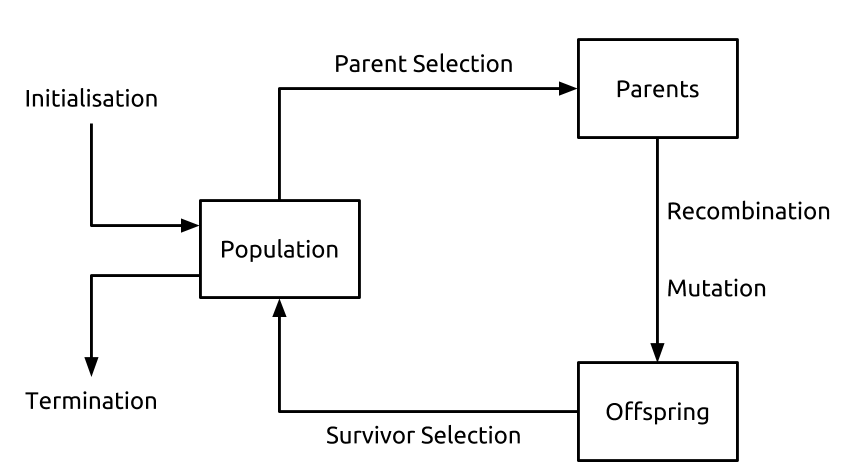
\includegraphics[scale=0.08]{./Figures/eaflowchart.png}
    \rule{20em}{0.5pt}
    \caption{The general scheme of an evolutionary algorithm as a flow-chart \cite{Eiben}}
    \label{fig:eaflowchart}
\end{figure}
The driving forces of evolutionary algorithms are the genetic operators, which are generating new diverse candidate solutions (novelty), and the natural selection, which is guiding to better candidate solutions (quality)\cite{Eiben}.\\
By preserving the possibility that candidate solutions with a lower fitness can be selected as seed for the offspring, the chance of getting into a local optimum should be minimized like in other meta-heuristics.\\

    \subsection{Components of Evolutionary Algorithms}
    An EA is defined by its components, procedures and operators, which will be briefly introduced in the following.
    \begin{itemize}
        
        \item \textbf{Individuals}\\
        The individuals of a population in EA represent candidate solutions. The candidate solutions within the original problem context are called phenotypes, while their representation in the EA are called genotypes or chromosomes. A building block of a chromosome is called a gene, where the possible values for a gene are called alleles. The mapping from the phenotype to the genotype is called encoding and the inverse mapping is called decoding. A representation could be for example a binary string or a string with real values. Both also more complex structures could be the right representation. Finding the right representation of the phenotypes is a difficult task and is crucial for the success of the EA. It also has an impact on the recombination and mutation operators.
        
        \item \textbf{Population}\\
        The population is a a list of individuals (genotypes), which can occur several times within the list. The individuals are static objects, which do not change. The population is dynamic, which will change over time due to the exchange of individuals. The parent selection of the individuals, which will be the seed for the offspring, is mostly carried out on the whole population size. In most EAs the population size remains constant. The diversity of a population describes the measure of how many different individuals are present. The measure can be based on the fitness values, the phenotypes or the genotypes of the individuals. For example two individuals can represent two different phenotypes, but are evaluated with the same fitness value.\\
        The first population consists of randomly generated individuals or of chosen individuals with higher fitness.
        
        \item \textbf{Evaluation Function (or Fitness function)}\\
        The evaluation function evaluates the individuals of a population and assigned the fitness of a candidate solution. Since the fitness influences the selection of an individual, the evaluation function encourages improvements. The goal could be to minimize or to maximize the fitness of individuals. Mathematically a minimization function can be easily transformed to a maximization problem and vice versa. The evaluation function in an EA is constructed from the objective function in the phenotype space.
        
        \item \textbf{Parent Selection}\\
        The parent selection is the selection of individuals, which will be the seed for the next generation. Typically individuals with a better fitness value get more often selected to further improve the individuals. But also individuals with a low quality fitness get a chance to pass on their genes into the next generation. This ensures that the search is not too greedy and get into a local optimum. The balance between parents with a high-quality fitness and parents with a low-quality fitness is often probabilistic.
           
        \item \textbf{Variation Operators (Recombination and Mutation)}\\
        The variation operators are responsible for discovering the search space by creating new individuals on the bases of existing individuals in the current population. All newly created individuals of a generation is called the offspring.\\
        There are different types of variation operators. While the mutation oparator only takes one individual as input, the recombination (or crossover) operator takes at least two individuals as input. The mutation operator creates a new individual (mutant), which slightly differs from the input-individual (original). The change from the original to the mutant is chosen randomly. If the change is not random but rather guided, it is defined as an heuristic operator. The recombination operation is creating one or more new individuals (children) from its parent individuals by mixing randomly genes of these. A child might have a lower, equal or higher fitness value than its parents depending on the combination of genes.\\
        Variation operators are depending on the representation of the phenotypes.
        
        \item \textbf{Survivor Selection (Replacement)}\\
        The survivor selection is the replacement strategy of the population and happens after the creation of the offspring. The current population is replaced by a new population - the new generation - which is mostly the same size as the population, which is being replaced. Like in the parent selection, the selection is based on the fitness values of the individuals and is often deterministic. In a fitnesss-biased selection for example the individuals of the population and the offspring are sorted by their fitness values and then the top segment is selected for the next population generation. In an age-biased selection only the individuals from the offspring are considered for the new population generation. If the current fittest individual of a population is kept in the next population, the concept of elitism is used.
        
        \item \textbf{Termination Condition}\\
        The EA is either terminated when one individual is reaching a known optimal fitness value or when predefined computation conditions are met. These conditions can be for example the number of generations, number of fitness evaluations, maximum allowed CPU time or a threshold under which the population diversity has to fall.
    \end{itemize}
        
    \subsection{Multi-Objective Genetic Algorithms}
    A problem might have not only one objective but several objectives. It is unlikely that there is one optimal solution, which is considered optimal for each single objective. It is rather likely to have a set of optimal solutions, where the solutions are optimal in respect to all objectives combined. This set of optimal solutions is also known as Pareto-optimal solutions.
    
    \begin{itemize}
        \item NSGA2\\
        Why? The higher the role number (1 Role for each user), the more likely it is to have no violations. The lower the role number, the more violations
        \item Improved NSGA2 (Fortin)\\
        Why? Different Individuals have same fitness
        \item Weighted NSGA2\\
        Why? 2nd objective is less important\\
        Issue? Skipped fronts, no symmetry in domination matrix
    \end{itemize}
    
    \subsection{Co-Evolution}
    \subsubsection{Symbiotic, Adaptive Neuro-Evolution (SANE)}
    \subsubsection{Enforced Sub-Populations (ESP)}
    
    \subsection{Human interaction}